% Chapter 3

\chapter{Onderzoeksmethode}\label{ch:onderzoeksmethode} % Chapter title

\label{OnderzoeksMethode} % For referencing the chapter elsewhere, use \autoref{ch:InOnderzoek}
Zoals in de inleiding vermeld zijn er twee onderzoek benodigd om deze opdracht tot een goed einde te brengen.
Voor ieder onderzoek wordt in dit hoofdstuk uitwijd over de methoden die zijn toegepast om antwoorden te verkrijgen op de vragen die opgekomen zijn na de requirements analyse.
\section{Onderzoeksmethode Architectuur binnen eagleScience}\label{sec:onderzoeksmethode-architectuur-binnen-eaglescience}

\subsection{Doel van het onderzoek}\label{subsec:doel-van-het-onderzoek}
Het doel van het onderzoek is het in kaart brengen van de werkwijze, de gebruikte architectuur en dev-stack die op dit moment wordt gebruikt binnen Eaglescience.
Daarnaast zal er ook een beeld worden gevormd welke tooling er dagelijks wordt gebruikt.
Deze informatie is nodig om een goede basis te vormen voor de ontwikkeling van de SOUP-Module in de bestaande portal.

\subsection{Onderzoeksmodel \ Strategie}\label{subsec:onderzoeksmodel--strategie}
Hieronder is het onderzoeksmodel te vinden waarbij aan de linkerzijde alle voorziene input staat voor het onderzoek en middels confontatie fase(tweede kolom) en consolidatie / reviewfase( derde kolom) tot een resultaat komt.
Om tot een resultaat te komen is de volgende strategie bedacht:
\begin{enumerate}
  \item Stel een onderzoeksvraag op en formuleer deelvragen die samen tot het gewenste antwoordt komt.
  \item Interviews met senior developers binnen Eaglescience.
  \item Interview met CTO
  \item Verwerk input tot een verslag geschikt voor naslag werk in verdere werkzaamheden aan de SOUP-Module
\end{enumerate}
\begin{figure}[h!]
\myfloatalign
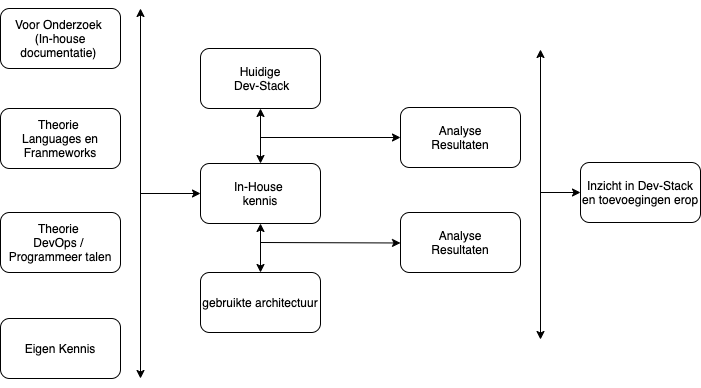
\includegraphics[width=10cm]{gfx/OnderzoeksmodelES}
\caption{Onderzoeksmodel Eaglescience}
\label{fig:Onderzoeks model Eaglescience}
\end{figure}


\section{Onderzoek naar SOUP analyse}\label{sec:onderzoek-naar-soup-analyse}

\subsection{Doel van het onderzoek}\label{subsec:doel-van-het-onderzoek2}
Het doel van dit onderzoek is het opbouwen van een theoretische basis voor het ontwikkelen van de SOUP module.
Alsmede methodes om dit geautomatiseerd te kunnen doen in combinatie met databases waar kwetsbaarheden in opgeslagen zijn.


\subsection{Onderzoeksmodel}\label{subsec:onderzoeksmodel}
Het onderstaande onderzoeksmodel is samengesteld uit de vragen aan de linkerkant en de weg naar het resultaat van links naar rechts.\\
\begin{figure}[h!]
\myfloatalign
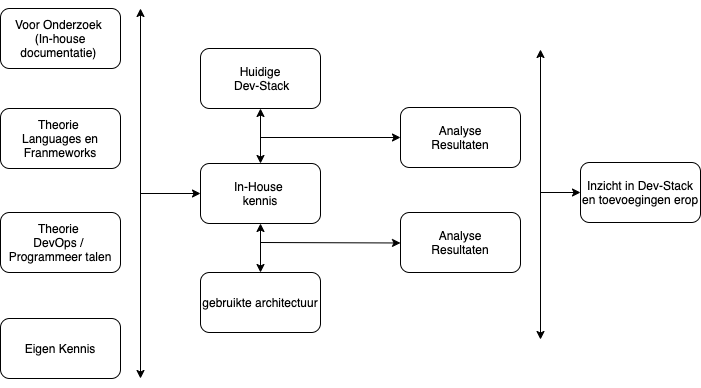
\includegraphics[width=10cm]{gfx/OnderzoeksmodelES}
\caption{Onderzoeksmodel SOUP analyse module}
\label{fig:Onderzoeks model Dev-Stack}
\end{figure}

\subsection{Onderzoeks vragen}\label{subsec:onderzoeks-vragen}
De hoofdvraag in dit onderzoek luid: \\
"Waaruit bestaat de huidige Dev-stack en welke tooling missen we om een geautomatiseerde SOUP analyse te doen?"\\
Uit deze hoofdvraag komen een aantal deelvragen:

\begin{itemize}
  \item Hoe wordt op dit moment gewerkt binnen Eaglescience en dan met name op het gebied van SOUP analyses?
  \item Welke Ontwikkeltalen gebruiken we binnen Eaglescience?
  \item Welke frameworks worden er gebruikt binnen de ontwikkeltalen?
  \item Hoe wordt op dit moment de ontwikkelde software gedeployed?
  \item Welke architectuur wordt er op dit moment gebruikt in de portal?
  \item Waar wordt de softwar uiteindelijk gedeployed?
  \item Nog veel meer vast??
\end{itemize}

\subsection{Resultaat}\label{subsec:resultaat}% is dit niet het zelfde als het doel.
Het resultaat van dit onderzoek moet zijn dat er een theoretische basis is voor het verdere verloop van het project.
\subsection{Strategie}\label{subsec:strategie}
Dit onderzoek is voor een groot deel een bureauonderzoek uit bronnen online en boeken.
Waarbij er een verslag wordt gelegd die geverifieerd wordt door de opdrachtgever..
De beste manier om de antwoorden op deze vragen te krijgen is door het interviewen van de ontwikkelaars en de CTO. Deze hebben op dit moment de meeste kennis van de gebruikte systemen binnen Eaglescience.
Ook de verschillende "artifact files" (Package.json / build.sbt) zijn goede bronnen om te onderzoeken welke frameworks er gebruikt worden het gaat dan voornamelijk over de build tools waar informatie uit te halen is over bibliotheken en versies hiervan.

\section{Tijdsverloop Onderzoeken}\label{sec:tijdsverloop-onderzoeken}
Beide onderzoeken zullen parallel uitgevoerd worden zodat beide onderzoeken elkaar inzichten kunnen verschaffen en er op die manier een beter begrip van de mogelijkheden is.
